\documentclass{beamer}

\usepackage[utf8]{inputenc}
\usepackage[slovene]{babel}
\usepackage{default}
\usepackage{graphicx}
\usepackage{amsmath}
\usepackage{overpic}
\usepackage{geometry}
\usepackage{subfigure}
\usepackage{calc}

\renewcommand{\thesubfigure}{}
\setbeamertemplate{navigation symbols}{}

\usepackage{tikz}
\usetikzlibrary{calc}

\tikzset{egrid/.style={draw,help lines}}
\tikzset{mgrid/.style={draw,help lines,dashed}}
\tikzset{epoint/.style={draw,circle,red,inner sep=2pt,fill}}
\tikzset{mpoint/.style={draw,circle,blue,inner sep=2pt,fill}}

\usetheme{Madrid}

\newcommand{\odvod}[2]{\frac{\partial #1}{\partial #2}}
\renewcommand{\vec}{\mathbf}
\newcommand{\eps}{\varepsilon}
\newcommand{\E}{\vec E}
\newcommand{\B}{\vec B}
\newcommand{\angl}[1]{(\textit{angl. #1})}
\newcommand{\ticssize}{\fontsize{9}{10}\selectfont}

\newcommand{\stalno}[2]{
  \begin{overpic}[width=.23\textwidth,trim=-1cm -1cm -1cm -1cm]{g_defect_#2}\end{overpic} 
  \begin{overpic}[width=.23\textwidth]{./Slike/lic_#1_1}\put(2,88){\color{white} \large \bf 1 $\boldsymbol\mu$m}\end{overpic} 
  \begin{overpic}[width=.23\textwidth]{./Slike/lic_#1_37}\put(2,88){\color{white} \large \bf 10 $\boldsymbol\mu$m}\end{overpic} 	
  \begin{overpic}[width=.23\textwidth]{./Slike/lic_#1_50}\put(2,88){\color{white} \large \bf 15 $\boldsymbol\mu$m}\end{overpic}
}

\begin{document}
\title[Zagovor magisterija]{Modeliranje \v sirjenja svetlobe vzdol\v z ograjenih teko\v cekristalnih defektnih linij}
\author[Miha \v Can\v cula]{\begin{tabular}{rl}Avtor & Miha \v Can\v cula \\ Mentor & prof. dr. Slobodan \v Zumer \\ Somentor & doc. dr. Miha Ravnik\end{tabular}}

\date{3. september 2013}

\section{Uvod}

\begin{frame}
 \titlepage
\end{frame}

\begin{frame}{Teko"ci kristali}
 \begin{columns}[c]
  \begin{column}{.5\textwidth}
  
   \begin{itemize}
    \item Lastnosti teko"cin in kristalov
    \item Orientacijski red
      \begin{itemize}
	\item Direktor $\vec n$
	\item Stopnja reda $S$
	\item Simetrija $\vec n \leftrightarrow -\vec n$
      \end{itemize}
    \item Delni pozicijski red
    \item<2-> Dvolomnost
    \item<2-> Nadzor z zunanjimi polji
    \item<2-> Elasti"cne deformacije direktorja
   \end{itemize}
  \end{column}

  \begin{column}{.5\textwidth}
    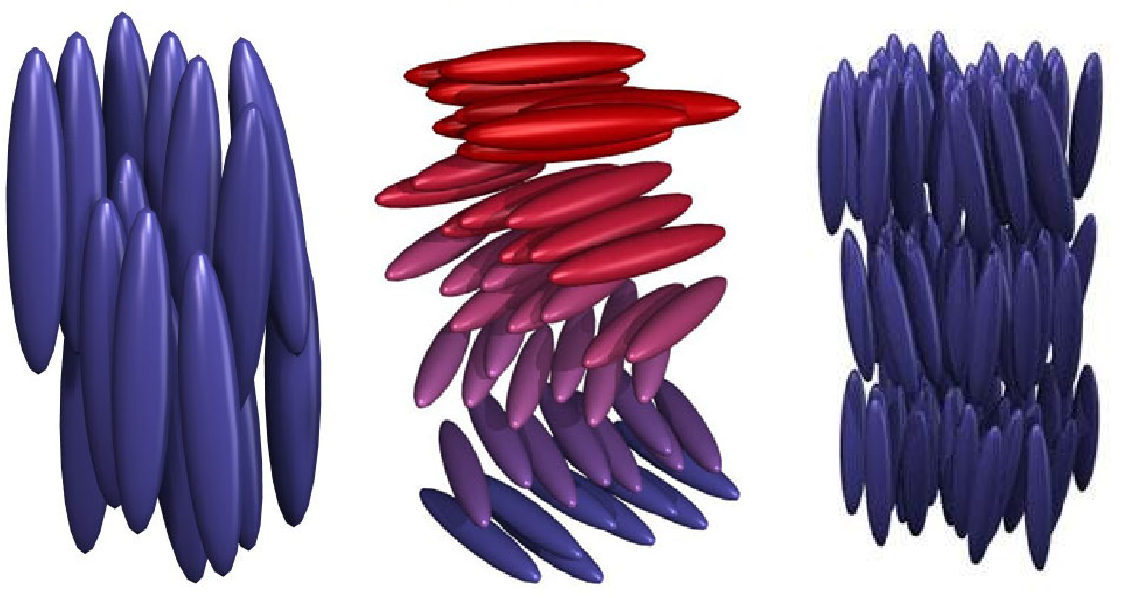
\includegraphics[width=\textwidth]{./Slike/faze_brez_crk} \\

  \resizebox{\textwidth}{!}{\begin{picture}(400, 120)
    \put(0,30){\includegraphics<2->[height=80pt]{./Slike/fig_frank_components_splay_s}}
    \put(150,20){\includegraphics<2->[height=100pt]{./Slike/fig_frank_components_twist_s}}
    \put(270,30){\includegraphics<2->[height=80pt]{./Slike/fig_frank_components_bend_s}}
    \put(50, 10){\only<2->{\LARGE $\nabla \cdot \vec n$}}
    \put(170, 10){\only<2->{\LARGE $\vec n \cdot \nabla \times \vec n$}}
    \put(300, 10){\only<2->{\LARGE $\vec n \times \nabla \times \vec n$}}
  \end{picture}}
  \end{column}
    
  \end{columns}
  
  \only<-2>{\vspace{54.5pt}}
  
  \begin{center}
   \includegraphics<3->[height=60pt]{./Slike/Flat-panel-display-lcd-monitor}\, 
   \includegraphics<3->[height=60pt]{./Slike/cp-1} \,
   \includegraphics<3->[height=60pt]{./Slike/dierking_june2013} \,
   \includegraphics<3->[height=60pt]{./Slike/tvorjenje}
  \end{center}

  
\end{frame}

\begin{frame}{Elektromagnetno valovanje}
\begin{columns}

\column{.6\textwidth}
 
\begin{block}{Maxwellove ena"cbe}
\begin{equation*}
\begin{aligned}
 \nabla \cdot \vec D = \rho_f & \qquad \nabla \cdot \vec B = 0 \\
 \nabla \times \vec E = -\odvod{\vec B}{t} & \qquad \nabla \times \vec H = \vec J_f + \odvod{\vec D}{t}
\end{aligned} 
\end{equation*}
\end{block}

\begin{block}{Konstitutivni zvezi}
\begin{equation*}
\begin{aligned}
\vec D = \boldsymbol\varepsilon \varepsilon_0 \vec E \qquad \vec B = \boldsymbol \mu \mu_0 \vec H
\end{aligned} 
\end{equation*}
\end{block}

\begin{itemize}
 \item $\boldsymbol\eps$ in $\boldsymbol\mu$ sta anizotropna tenzorja
 \item V vzorcu ni prostih nabojev ali tokov
 \item Izredna os in dvolomnost $\Delta n$ \\ v TK krajevno odvisna
\end{itemize}

\column{.35\textwidth}
\begin{block}{Dvolomnost}
\begin{itemize}
 \item Lomni koli"cnik odvisen od polarizacije svetlobe
 \item Ena izredna os z $n_e$ pravokotne smeri $n_o$
\end{itemize}
\end{block}

\begin{center}
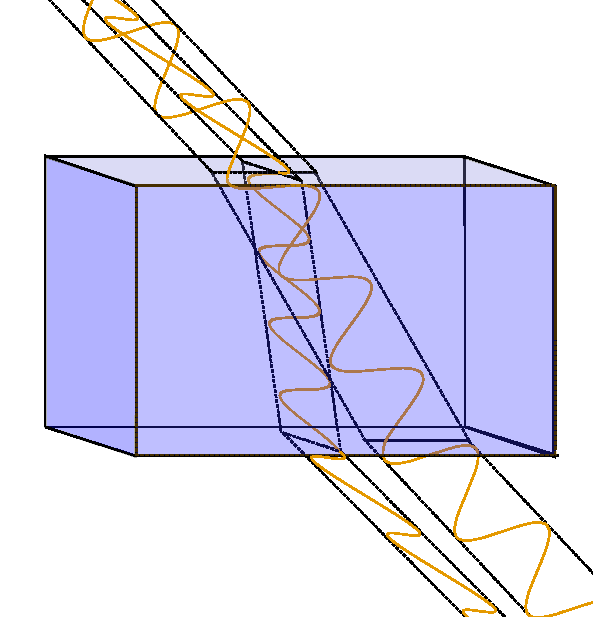
\includegraphics[width=.8\textwidth]{./Slike/Rays_passing_through_birefringent_material}
\end{center}

\end{columns}
\end{frame}

\begin{frame}{Topolo"ski defekti}
\begin{figure}
 \centering
 \subfigure[$s = +1$]{\includegraphics[width=.18\textwidth]{g_defect_2} \vspace{-2mm}}\,
 \subfigure[$s = -1$]{\includegraphics[width=.18\textwidth]{g_defect_-2} \vspace{-2mm}}\,
 \subfigure[$s = +1/2$]{\includegraphics[width=.18\textwidth]{g_defect_1} \vspace{-2mm}}\,
 \subfigure[$s = -1/2$]{\includegraphics[width=.18\textwidth]{g_defect_-1} \vspace{-2mm}}
 \end{figure}
 
 \vspace{-3mm}

 \begin{itemize}
  \item To"cka z nedefinirano smerjo direktorja ali elektri"cnega polja
  \item Ovojno "stevilo -- celo za vektorska polja, polcelo za direktor
 \end{itemize}
 
 \begin{center}
 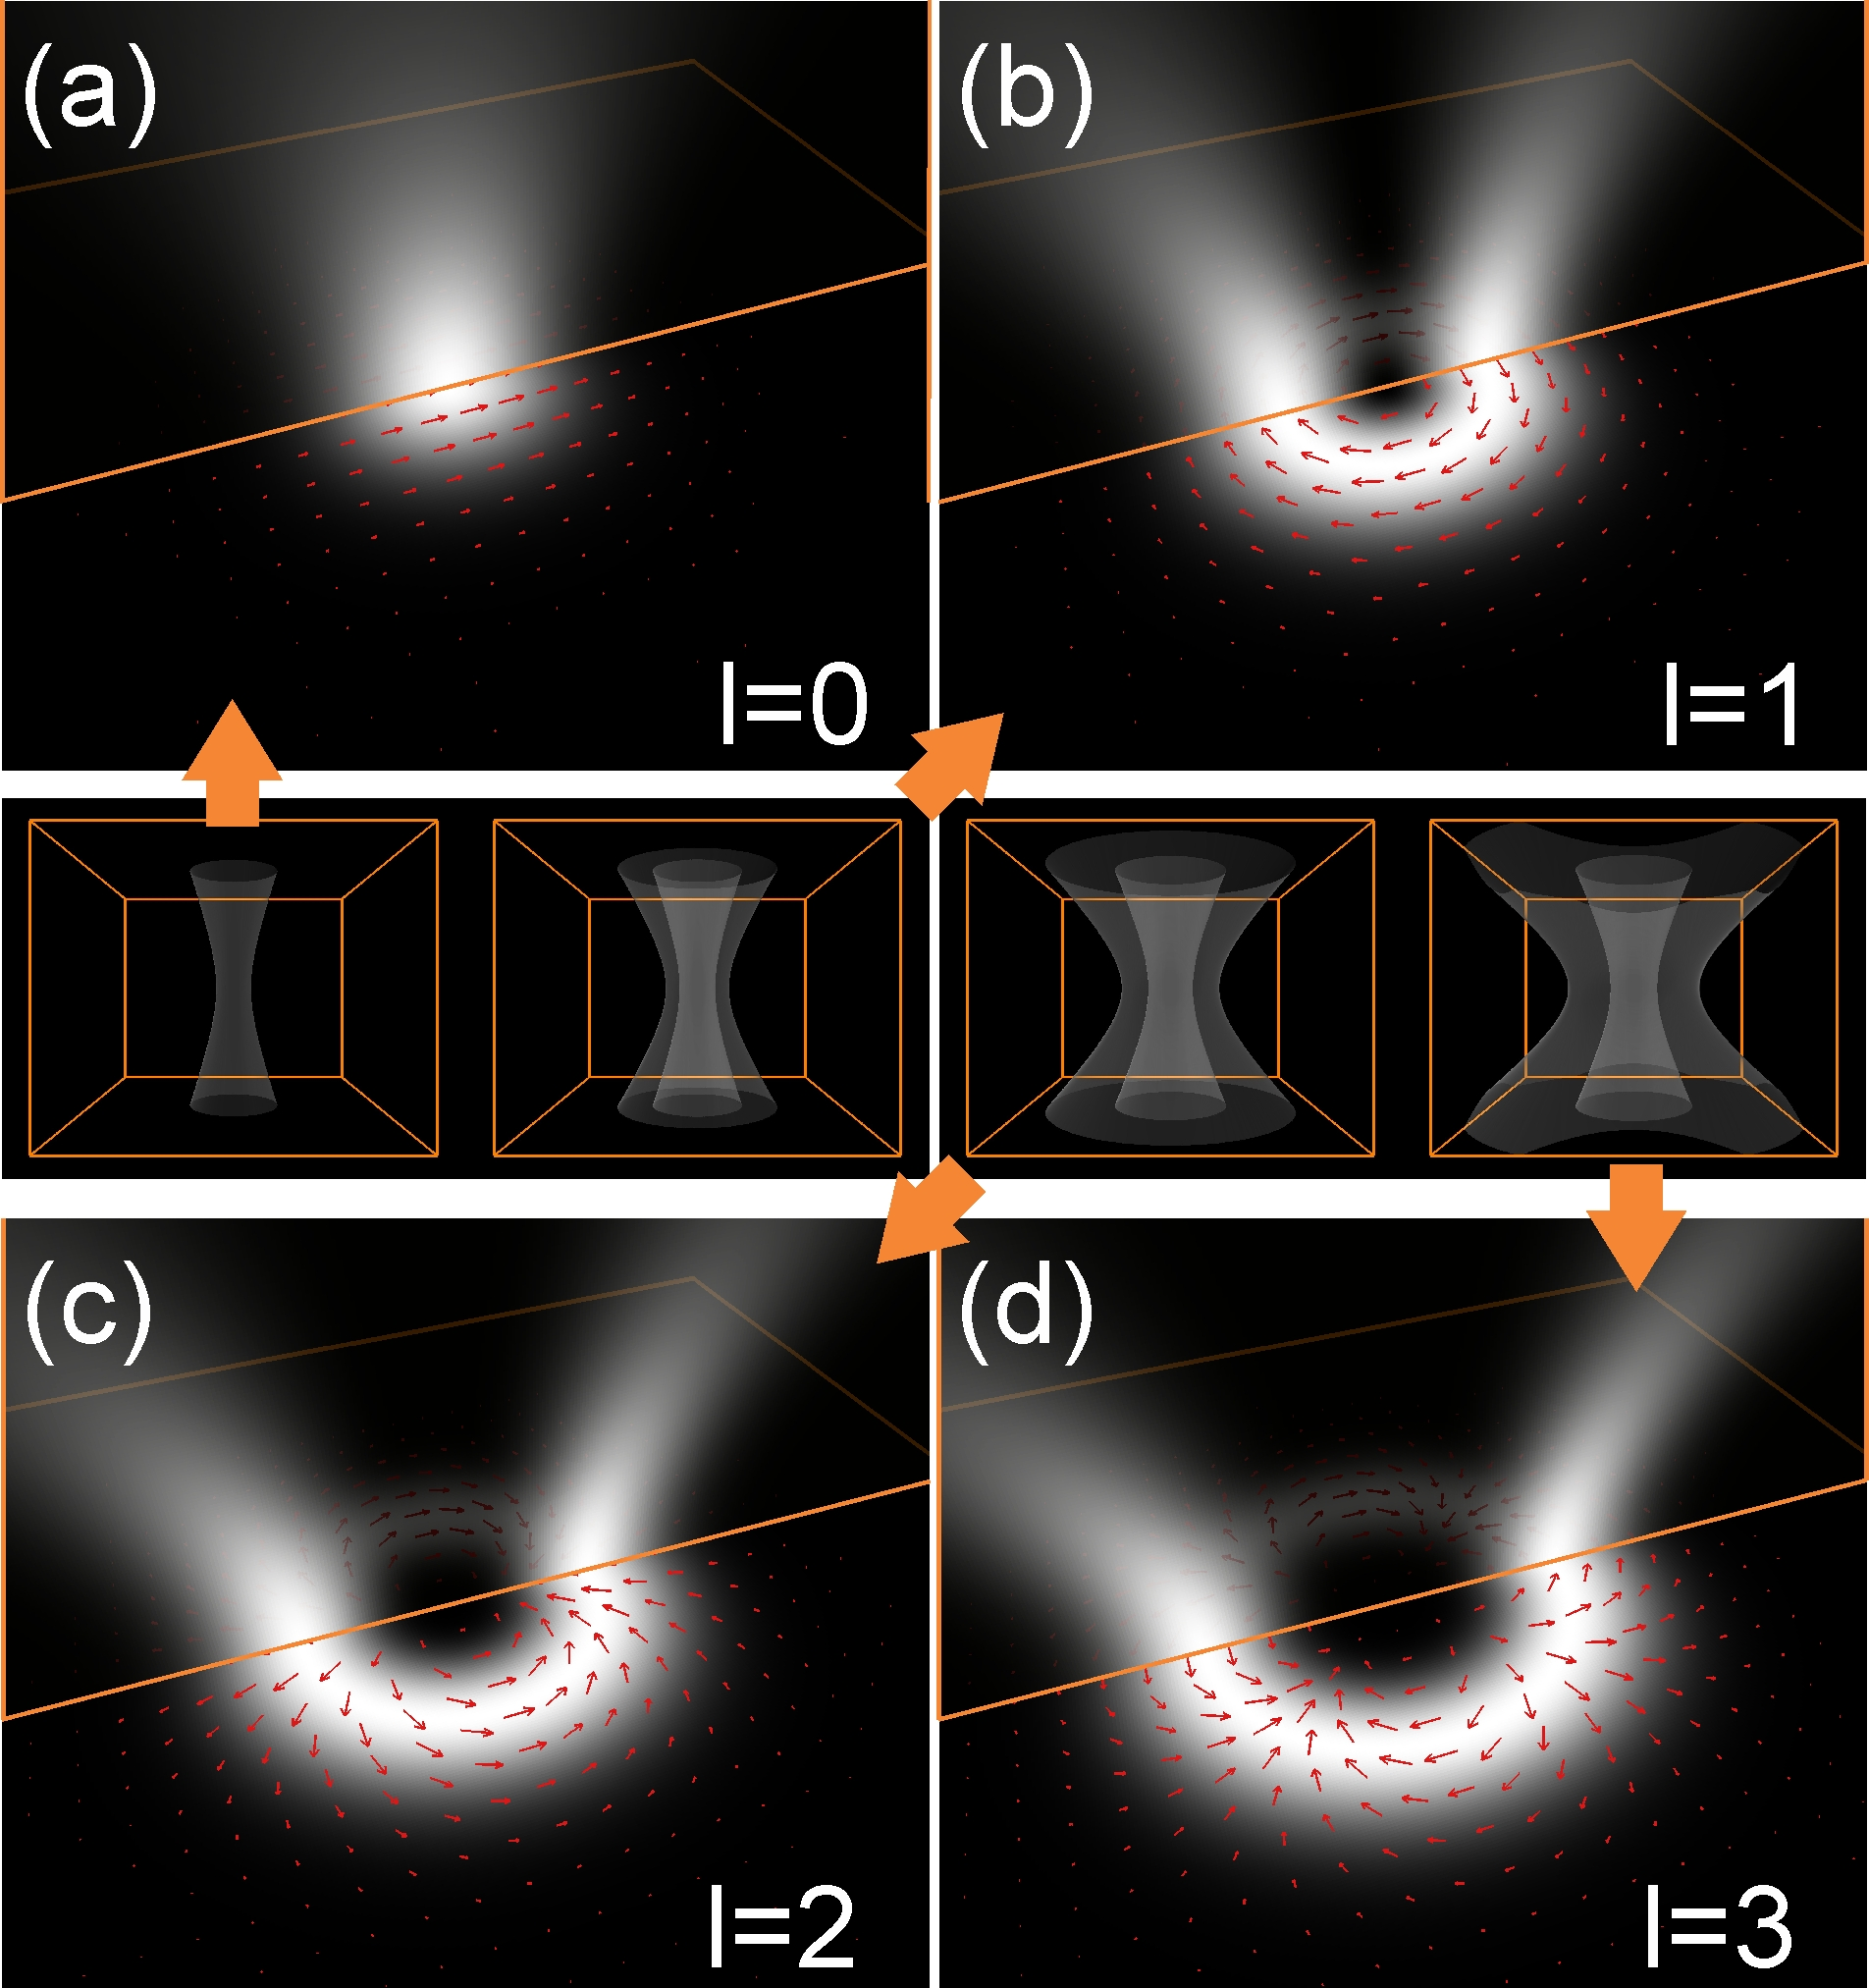
\includegraphics[height=100pt]{./Slike/1_v6} \qquad
 \begin{overpic}[height=100pt]{./Slike/defekt-kapljica.png}
  \put(-80,4) {\rotatebox{90}{\tiny Porenta et al., Soft Matter (2012)}}
  \put(10,15) {\tiny Brasselet et al., PRL (2009)}
  \end{overpic}

 \end{center}
 
\end{frame}

\section{Metoda}

\begin{frame}{Numeri"cna metoda}
 \begin{block}{Metoda kon"cnih diferenc v "casovni domeni -- FDTD}
  \begin{itemize}
   \item "Casovni razvoj vseh 6 komponent $\vec E$ in $\vec B$
   \item Dinami"cni Maxwellovi ena"cbi na diskretni mre"zi
   \begin{equation*}
     \odvod{\vec{B}}{t} = -\left(\nabla \times \vec{E}\right) \qquad \odvod{\vec{E}}{t} = \boldsymbol\eps^{-1} \, \left(\nabla \times \vec{B}\right)
   \end{equation*}
  \end{itemize}
 \end{block}
 
 \begin{columns}
  \column{.65\textwidth}
   \begin{block}{Diskretizacija na mre"zi}
    \begin{itemize}
	\item Komponente polj znane na razli"cnih krajih ob razli"cnih "casih
	\item Izvor in absorpcija valovanja na robu
      \end{itemize}
    \end{block}
    
    \column{.3\textwidth}
    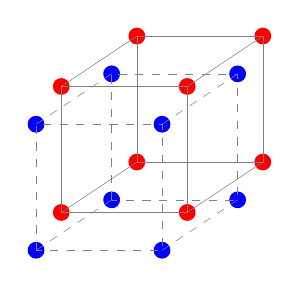
\begin{tikzpicture}[scale=0.8]
    
    \foreach \x in {0,1}{
      \foreach \y in {0,1}{
        \node[mpoint] at (2*\x,2*\y) {}; 
        \node[mpoint] at (2*\x+1.2,2*\y+0.8) {}; 
        \node[epoint] at (2*\x+1.6,2*\y+1.4) {};
        \node[epoint] at (2*\x+1.6-1.2,2*\y+1.4-0.8) {};
        \draw[mgrid] (2*\x,2*\y) -- (2*\x+1.2,2*\y+0.8);
        \draw[egrid] (2*\x+1.6,2*\y+1.4) -- (2*\x+1.6-1.2,2*\y+1.4-0.8);
      }
    }
    
    \draw[mgrid] (0,0) rectangle (2,2);
    \draw[mgrid] (1.2,0.8) rectangle (3.2,2.8);
    \draw[egrid] (1.6,1.4) rectangle (3.6,3.4);
    \draw[egrid] (1.6-1.2,1.4-0.8) rectangle (3.6-1.2,3.4-0.8);

            \end{tikzpicture}

 \end{columns}
\end{frame}

\begin{frame}{Simulacijska celica}
\begin{columns}
 
 \column{.5\textwidth}
 
 \begin{block}{Izvor valovanja}
 \begin{itemize}
  \item Delitev na dve obmo"cji
  \item Linearne ena"cbe $\rightarrow$ \\ vpadno + sipano valovanje
  \item Zunaj samo sipano valovanje
  \item Izvor modeliran na meji
 \end{itemize}
 \end{block}

 \column{.45\textwidth}
 \begin{center}
 
\includegraphics[width=.8\textwidth]{./Slike/wave-source-regions-one}
 \end{center}
 \end{columns}
 \begin{columns}

 \column{.45\textwidth}

 \begin{center}
 \includegraphics<2->[width=.9\textwidth]{./Slike/celica}
 \end{center}

  \column{.5\textwidth}

 \begin{block}<2->{Absorpcija na robu}
  \begin{itemize}
   \item Elektri"cna prevodnost in magnetne izgube
   \item Nefizikalen material -- \\ dodatne prostostne stopnje
  \end{itemize}
 \end{block}

\end{columns}
\end{frame}


\begin{frame}{Primeri uporabe metode}
\begin{columns}[c]

\begin{column}[T]{.46\textwidth}
\begin{itemize}[<+->]
 \item "Sirjenje po praznem prostoru
 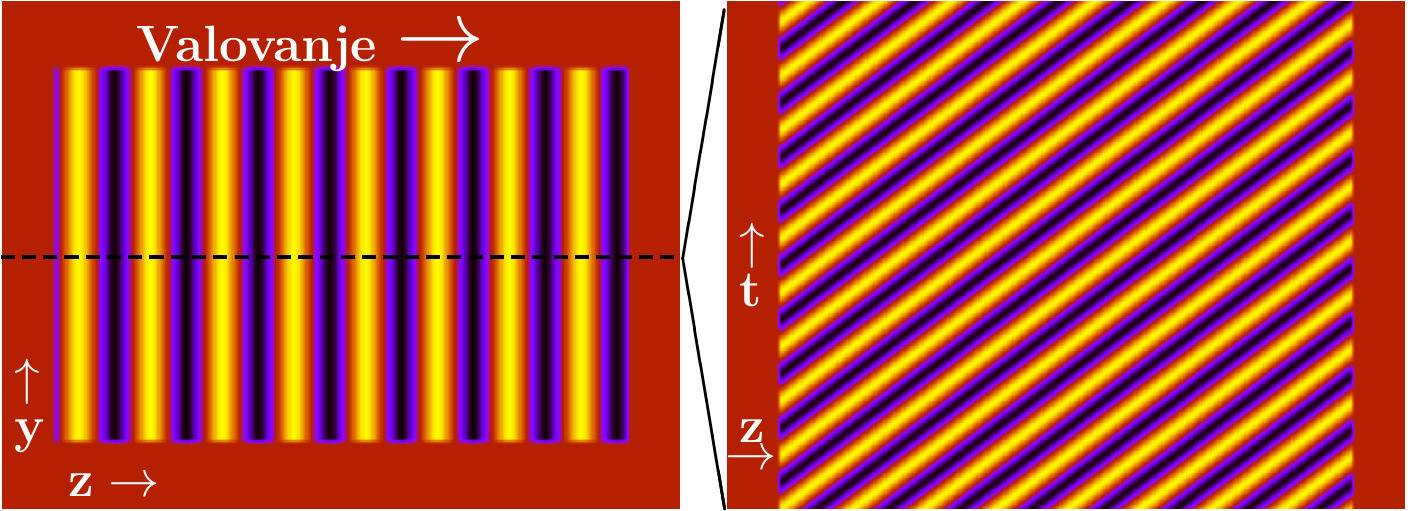
\includegraphics[width=.6\textwidth]{./Slike/empty}
 
 \item Lom pri Brewsterjevem kotu
 
\includegraphics[width=.6\textwidth]{./Slike/refraction}
 
 
  \item Dvolomni kristal med prekri"zanima polarizatorjema\\
  \resizebox{.65\textwidth}{!}{\input{g_test_uniform_nocite}}

\end{itemize}

\end{column}

\begin{column}[T]{.5\textwidth}
\begin{itemize}[<+->]
 \item Fotonski prepovedani pas
 \begin{center}
   \resizebox{.7\textwidth}{!}{\footnotesize \input{./Slike/bandgap.pdf_tex}} \\
    \hspace{-1cm} \raisebox{5mm}{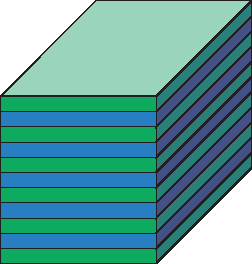
\includegraphics[width=.3\textwidth]{./Slike/periodic-structure-p}} \;	
  \resizebox{.6\textwidth}{!}{\input{g_test_periodic}}
  \end{center}
  
 \item Dvolomno vlakno \\
  \hspace{-0.6cm}
  \includegraphics[width=.29\textwidth]{./Defekti/g_defect_light_0} \,
  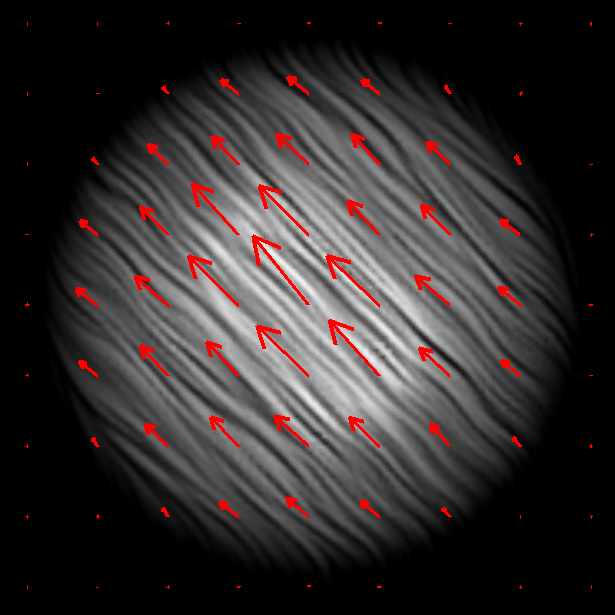
\includegraphics[width=.29\textwidth]{./Slike/licp_0_68} \,
  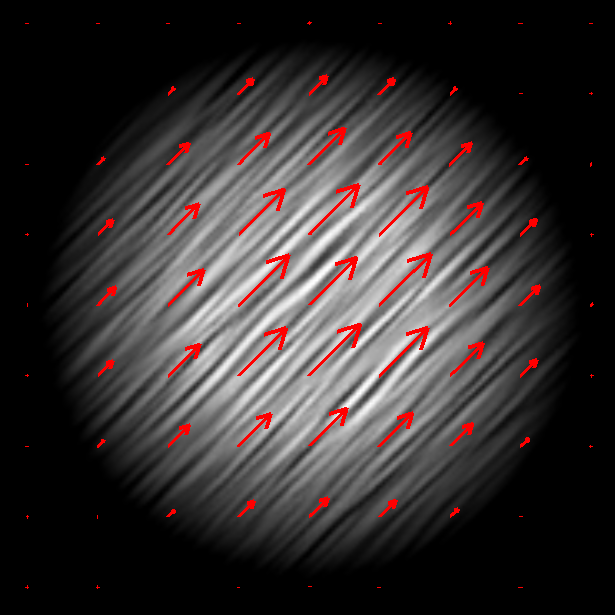
\includegraphics[width=.29\textwidth]{./Slike/licp_0_78}
\end{itemize}

\end{column}

\end{columns}

\end{frame}

\section{Rezultati}

\begin{frame}{Vlakno z radialnim direktorskim profilom}
 \begin{center}
 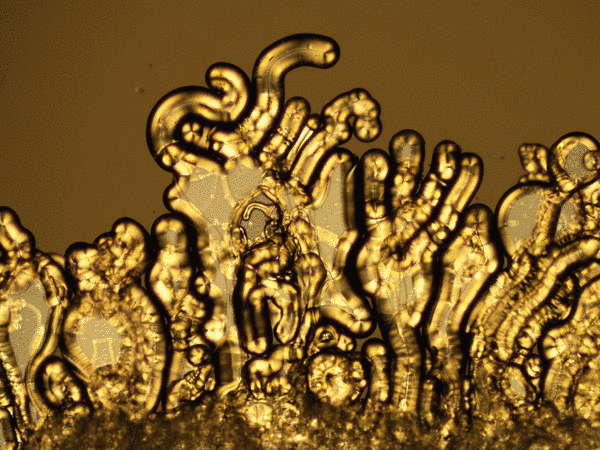
\includegraphics[height=.35\textwidth]{./Slike/tvorjenje}\,
 \begin{overpic}[height=.35\textwidth]{./Slike/tvorjenje2}
     \put(103, 10) {\rotatebox{90}{\tiny Peddireddy et al., Langmuir (2012)}}
\end{overpic}
\end{center}

\begin{columns}
 \column{.55\textwidth}
 
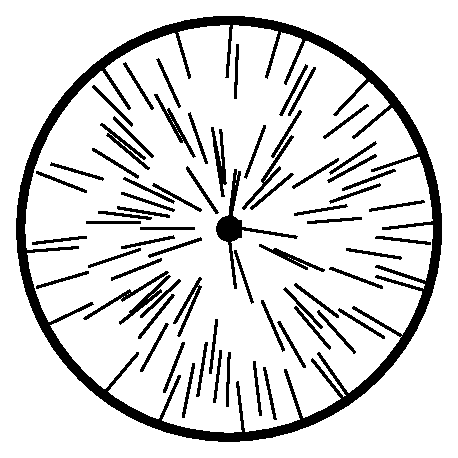
\includegraphics[height=.22\textwidth]{./Slike/radial-cross} \quad

\includegraphics[height=.22\textwidth]{./Slike/director-profile-radial} 

 \column{.3\textwidth}
 
\begin{itemize}
 \item Rast vlaken iz 8CB v vodi
 \item Delujejo kot valovodi
\end{itemize}

\end{columns}

\end{frame}

\begin{frame}{Sunek v vlaknu z radialnim direktorskim profilom}

 \begin{center}
 \raisebox{.075\textwidth}{\includegraphics[width=.2\textwidth]{./Defekti/g_defect_light_2}} \,
 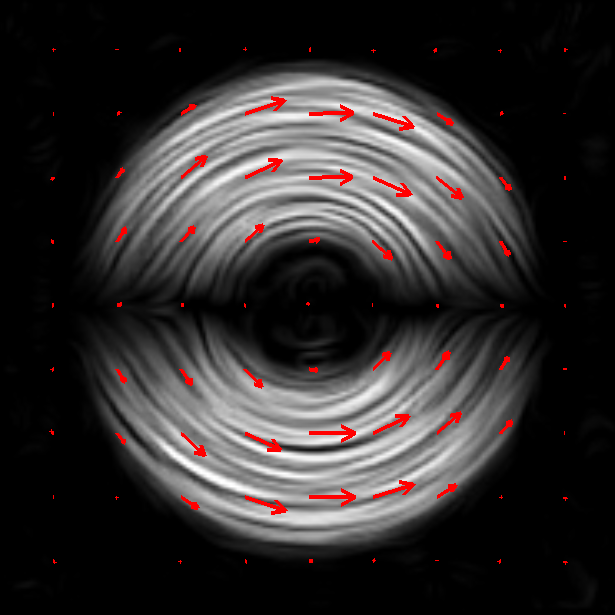
\includegraphics[width=.35\textwidth]{./Slike/licp_p1_74}\,
  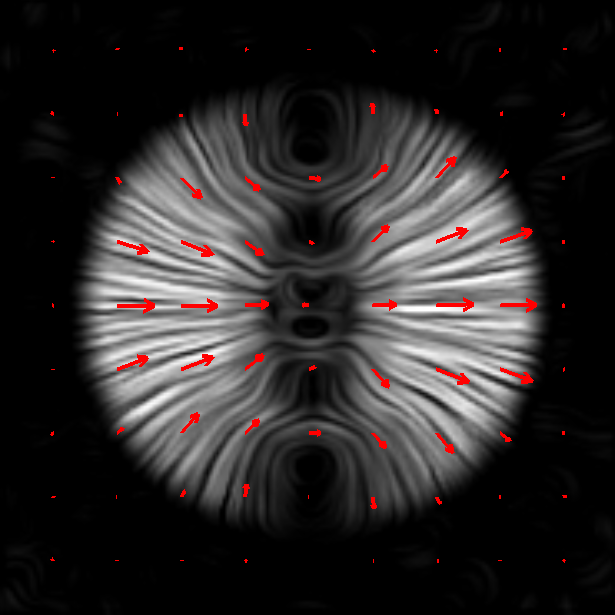
\includegraphics[width=.35\textwidth]{./Slike/licp_p1_82}
\end{center}

\begin{itemize}
 \item Sunek razpade na dva stacionarna na"cina -- redni in izredni
 \item ``Neprava'' defekta v $\vec E$ z ovojnim "stevilom $+1$
 \item Temna obmo"cja zaradi vpadne polarizacije
\end{itemize}

\end{frame}

\begin{frame}{Sunek v vlaknih z razli"cnimi defekti}

\begin{columns}

\column{.2\textwidth}
  \centering
  \includegraphics[width=.7\textwidth]{./Defekti/g_defect_light_-2} \\[2mm]
  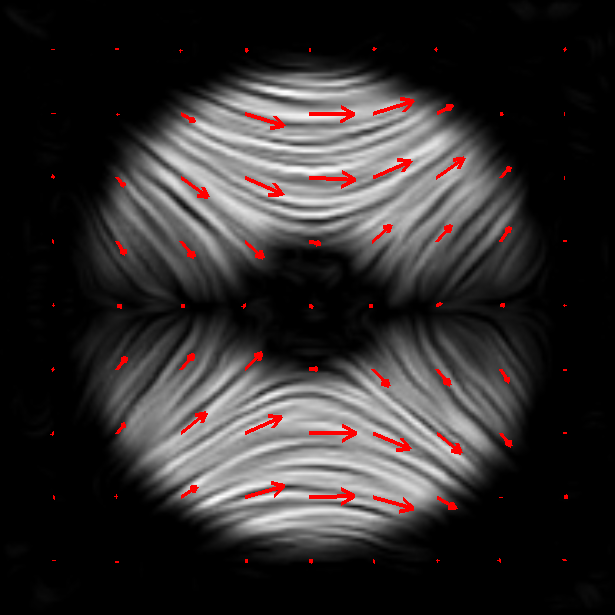
\includegraphics[width=\textwidth]{./Slike/licp_m1_74} \\[2mm]
  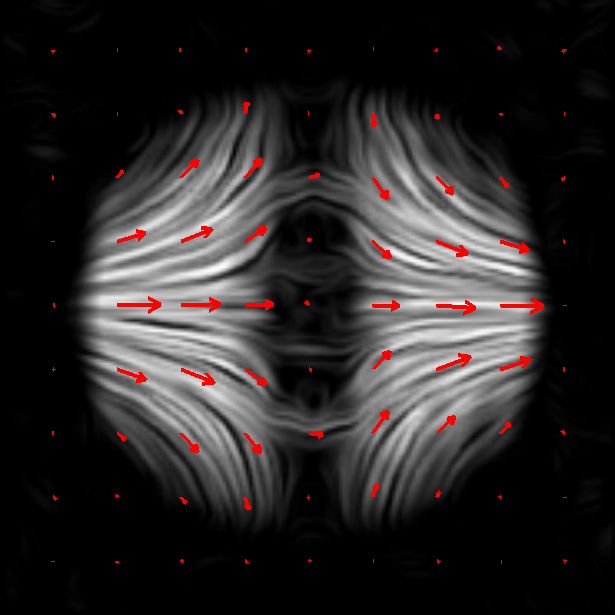
\includegraphics[width=\textwidth]{./Slike/licp_m1_82}
    
  \column{.2\textwidth}  
\centering
  \includegraphics[width=.7\textwidth]{./Defekti/g_defect_light_1} \\[2mm]
  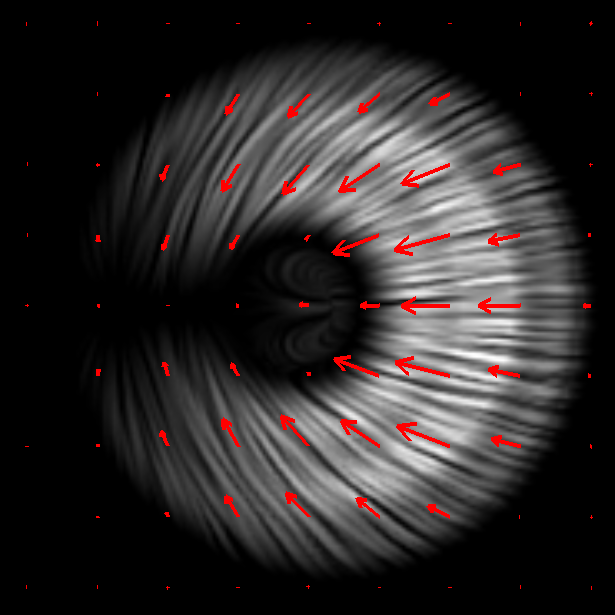
\includegraphics[width=\textwidth]{./Slike/licp_p12_68} \\[2mm]
  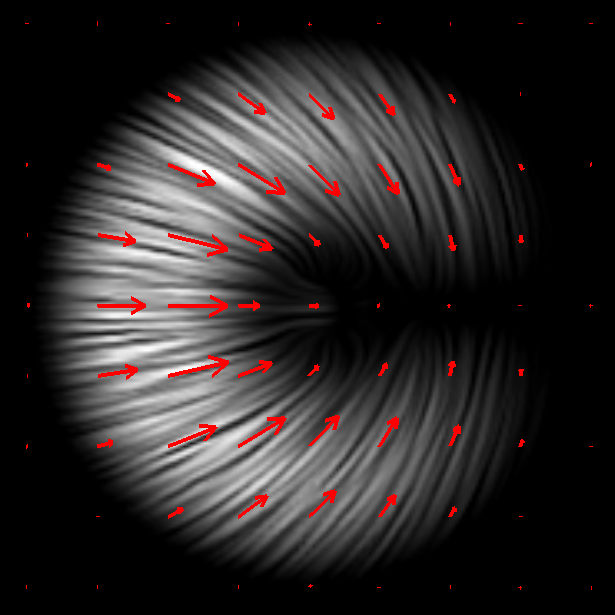
\includegraphics[width=\textwidth]{./Slike/licp_p12_78}
    
    \column{.2\textwidth}
\centering
  \includegraphics[width=.7\textwidth]{./Defekti/g_defect_light_-1} \\[2mm]
  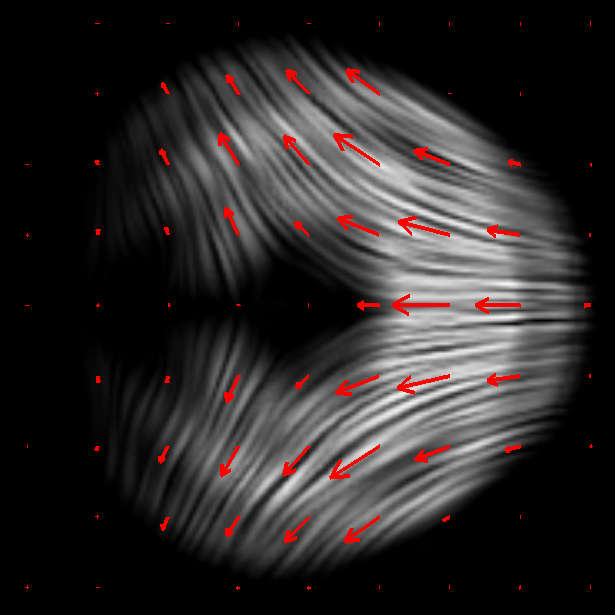
\includegraphics[width=\textwidth]{./Slike/licp_m12_68} \\[2mm]
  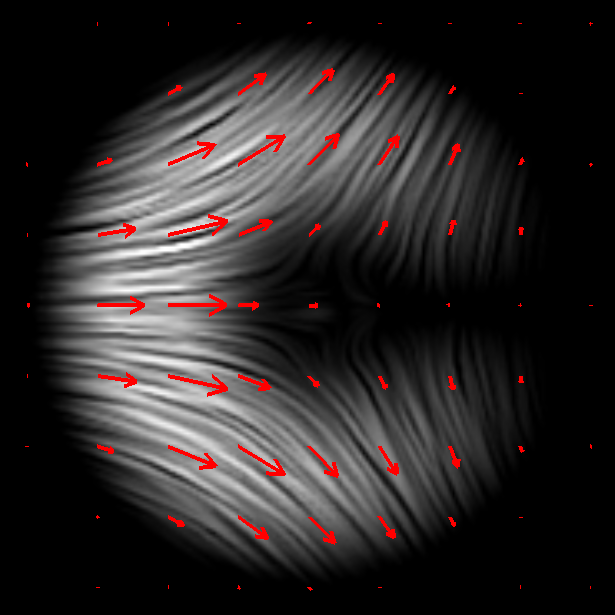
\includegraphics[width=\textwidth]{./Slike/licp_m12_78}
  
  \column{.35\textwidth}
  \begin{block}{Parametri}
  \begin{itemize}
   \item   $\lambda = 480$ nm
    \item $\Delta n = 0,\!16$
    \item Premer vlakna 5 $\mu$m
    \item Pot sunka $\sim 40$ $\mu$m
  \end{itemize}
    \end{block}
    
    \begin{block}{Opa"zanja}
     
\begin{itemize}
    \item 2 stacionarna na"cina
    \item Enako ovojno "stevilo kot defekt v TK
    \item Temna pega v osi
    \item Temne ravnine
  \end{itemize}
    \end{block}



  \end{columns}
\end{frame}

\begin{frame}{Stalna laserska svetloba}
\begin{itemize}
 \item Dvolomnost $\Delta n = 0,\!01$ $\Rightarrow$ ve"cja zna"cilna dol"zina pojavov
 \item Stacionarno stanje s krajevno odvisnostjo polarizacije
 \item Defekt z dvakratnim ovojnim "stevilom
\end{itemize}
  \stalno{p1}{2} \\[1mm]
  \stalno{p12}{1}
\end{frame}


\begin{frame}{Stalna laserska svetloba}
 \begin{itemize}
  \item Kombinacija dveh stacionarnih na"cinov, razli"cni hitrosti
  \item Stacionarno stanje, polje na vsakem mestu niha
  \item Pretvorba v radialno polarizirano svetlobo
  \item Brez temnih ravnin -- obrat polarizacije za 90$^{\circ}$
 \end{itemize}
 
 \begin{figure}[h]
 \centering
    \subfigure[sunek]{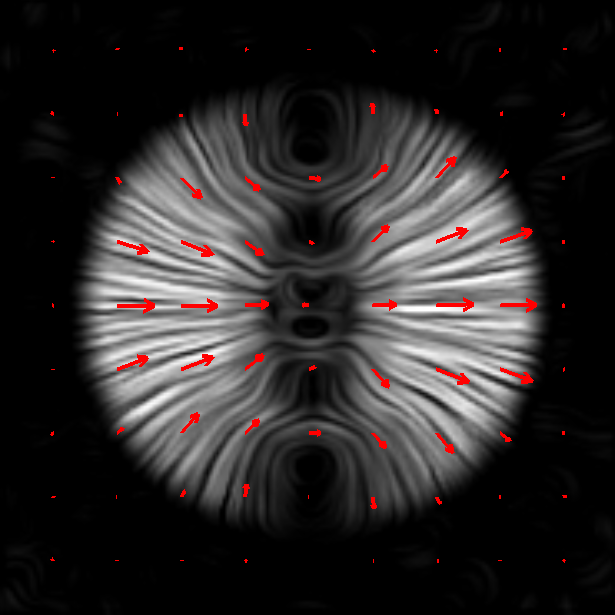
\includegraphics[width=.3\textwidth]{./Slike/licp_p1_82}} \hspace{.3cm}
    \raisebox{.13\textwidth}{\Huge $\boldsymbol\neq$} \hspace{.2cm}
    \subfigure[stalna svetloba]{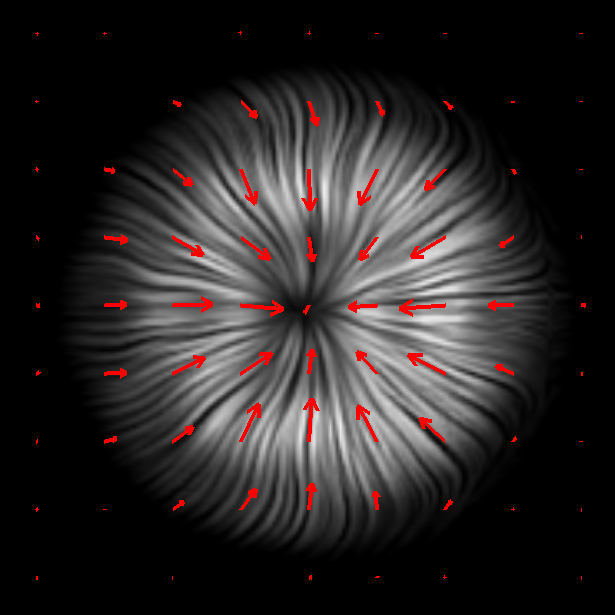
\includegraphics[width=.3\textwidth]{./Slike/lic_p12_50}}

    
 \end{figure}
  
\end{frame}

\section{Zaklju"cek}

\begin{frame}{Nadaljnje raziskave}
\begin{columns}

\column{.65\textwidth}
 
 \begin{block}{Teko"cekristalne strukture}
  \begin{itemize}
   \item Natan"cne transmisijske slike
   \item Povezava med teorijo in eksperimenti
   \item Pretvorba polarizacije svetlobe
   \item Teko"cekristalne kapljice in vlakna kot laserji
   \item Mikroskopija z bli"znjim poljem (\textit{near-field})
   \item Metamateriali, fotonski kristali, \ldots
  \end{itemize}
 \end{block}
 
 \begin{block}{Raz"siritev metode}
  \begin{itemize}
    \item Sklopitev med svetlobo in teko"cim kristalom
    \item Stimulirana emisija, fluorescenca
  \end{itemize}
 \end{block}
 
 
\column{.25\textwidth}

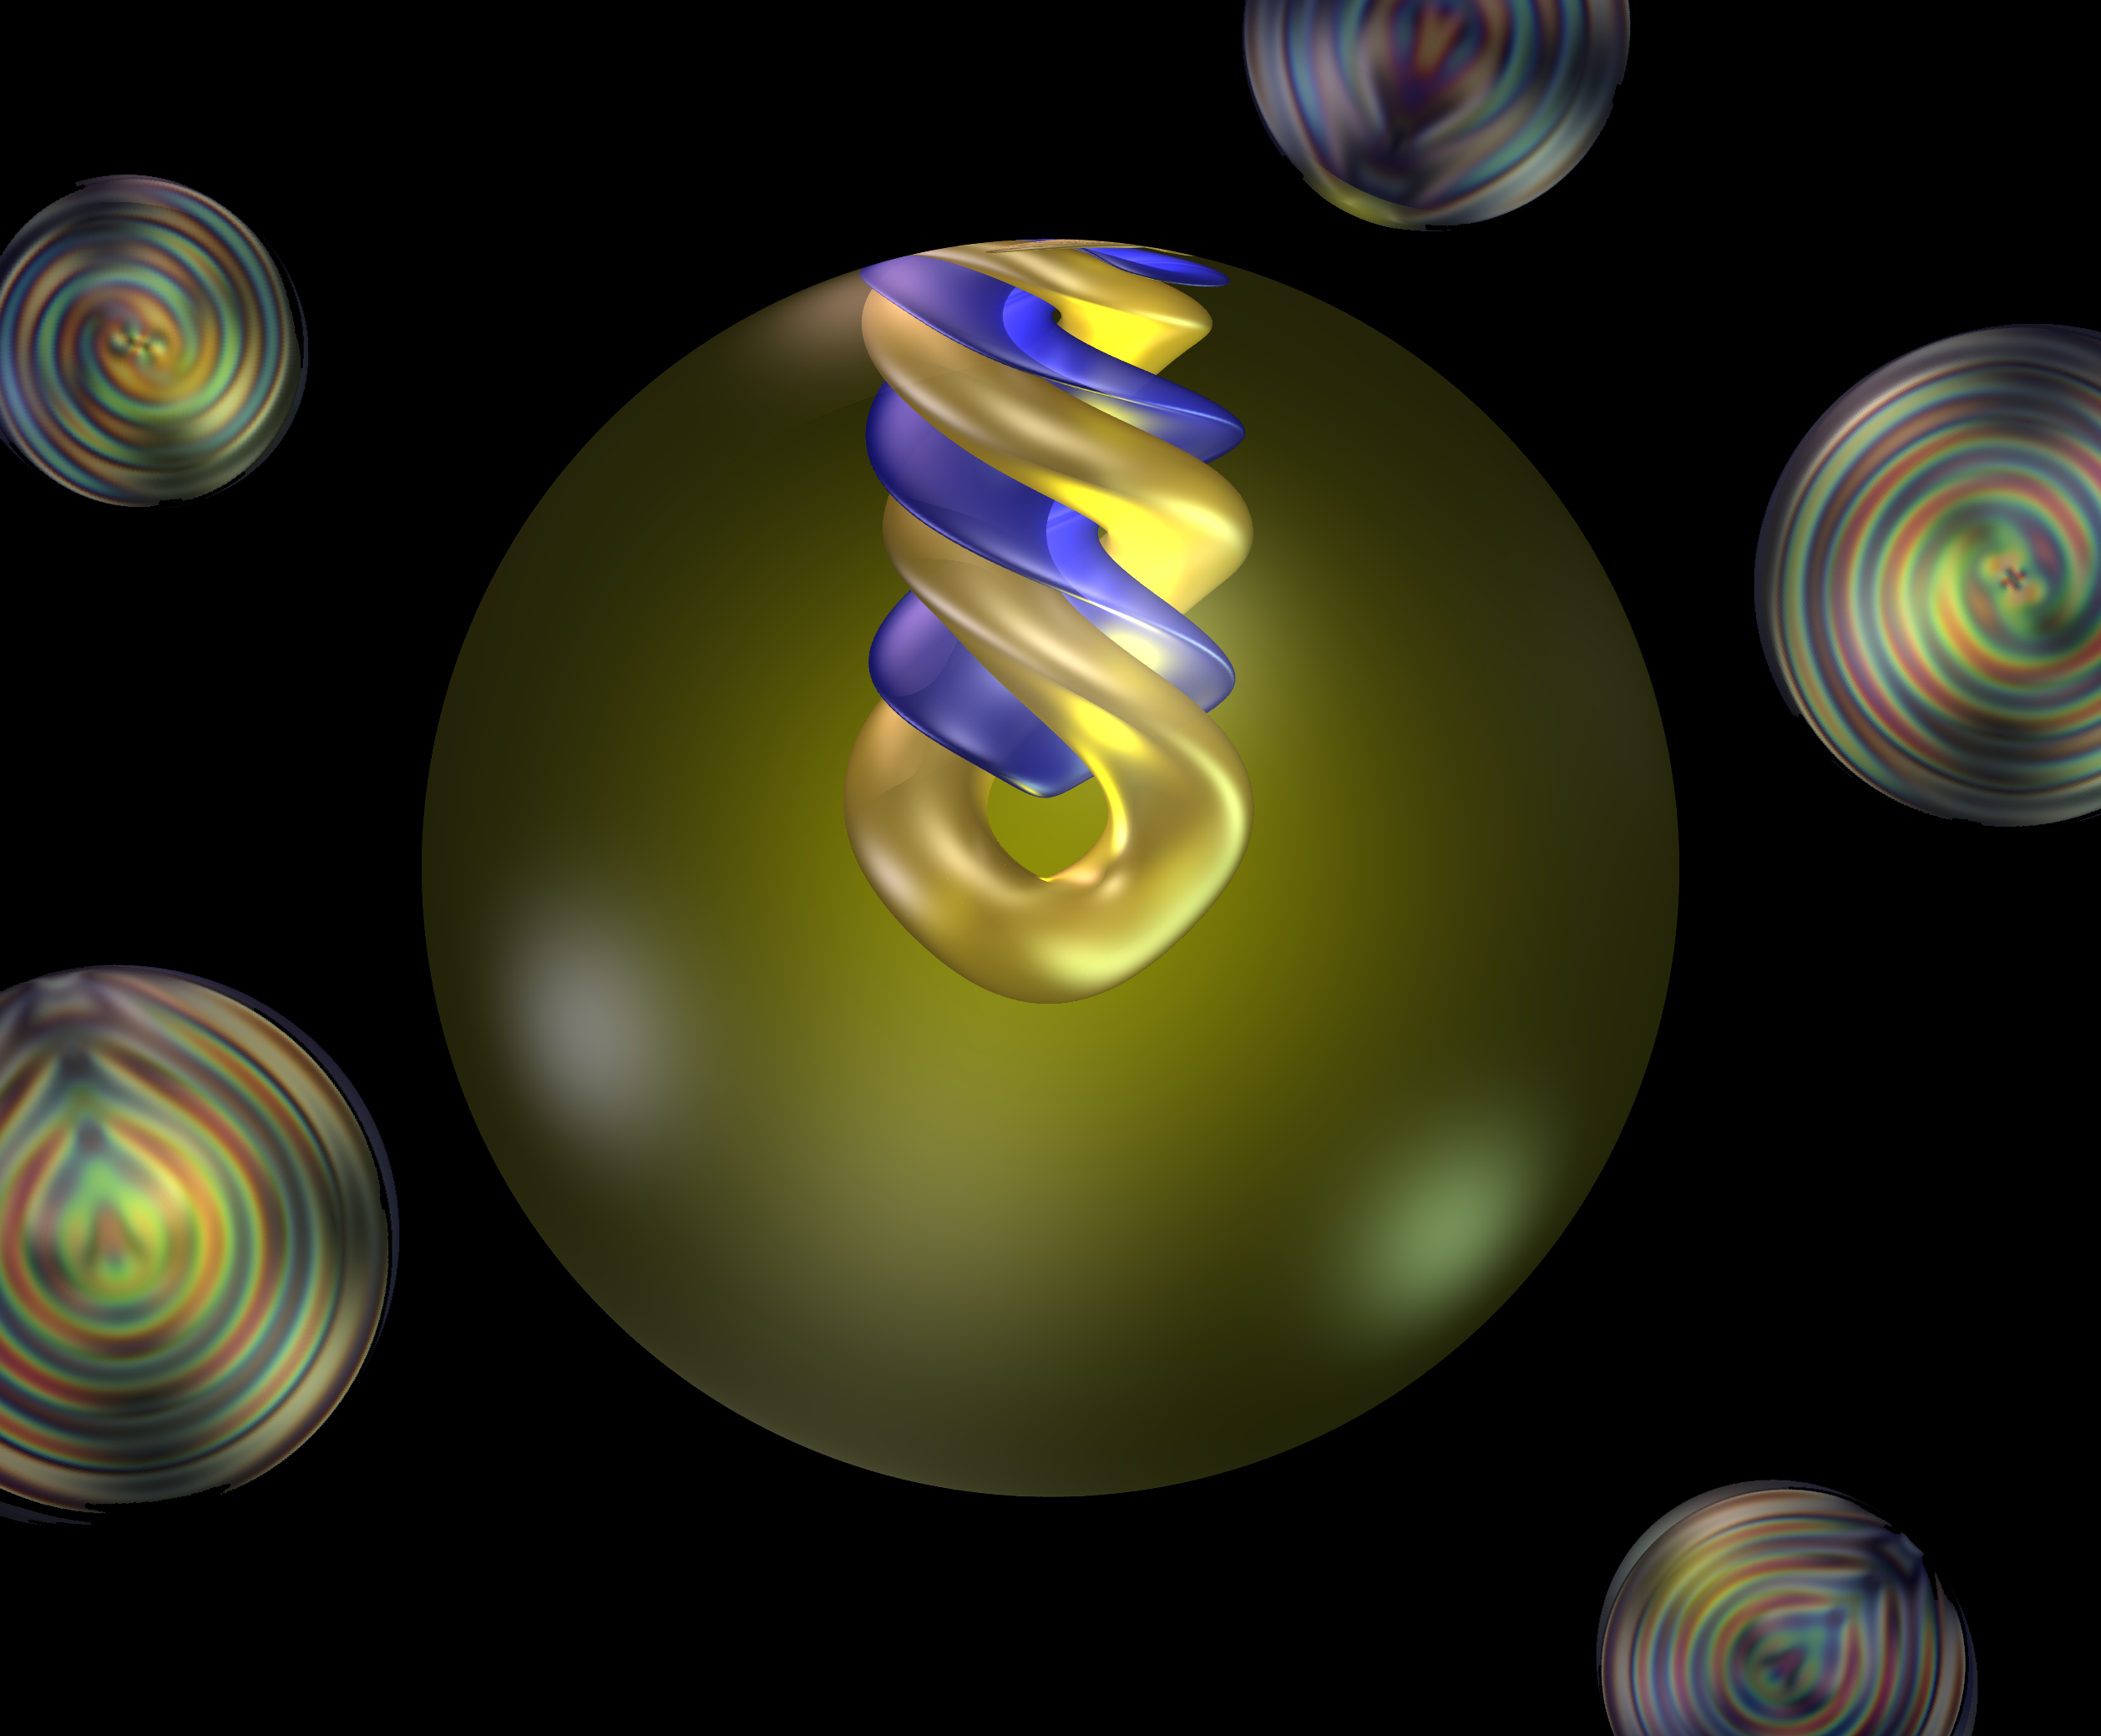
\includegraphics[width=\textwidth]{./Slike/s2-trans-noglare-noshine} \\[5mm]
\begin{overpic}[angle=90,width=\textwidth]{./Slike/laser-droplet}
\put(70,8) {\rotatebox{90}{\tiny Humar, Mu"sevi"c, Optics Express (2010)}}
\put(70,109) {\rotatebox{90}{\tiny Se"c et al., Soft Matter (2012)}}
\end{overpic}
 
\end{columns}
\end{frame}


\end{document}
